\section{去均值、去线性趋势和波形尖灭}
相关命令:\nameref{cmd:rmean}、\nameref{cmd:rtrend}、\nameref{cmd:taper}

通常,波形数据总会存在一个非零的均值或者存在一个长周期的线性趋势,这会影响到数据
的分析,必须在数据分析前去除。另一方面,在对数据进行谱域操作(如FFT、滤波等)时,
若数据的两端不为零,则会出现谱域假象,因而实际数据经常需要做尖灭处理,
使得数据两端在短时间窗内逐渐变成零值。

\begin{SACCode}
SAC> fg seis
SAC> rmean; rtr; taper
\end{SACCode}

图~\ref{fig:rmean-rtrend-taper}~中,波形从上到下依次为原始波形、去均值、去线性趋势、和尖灭之后的波形。

\begin{figure}[H]
\centering
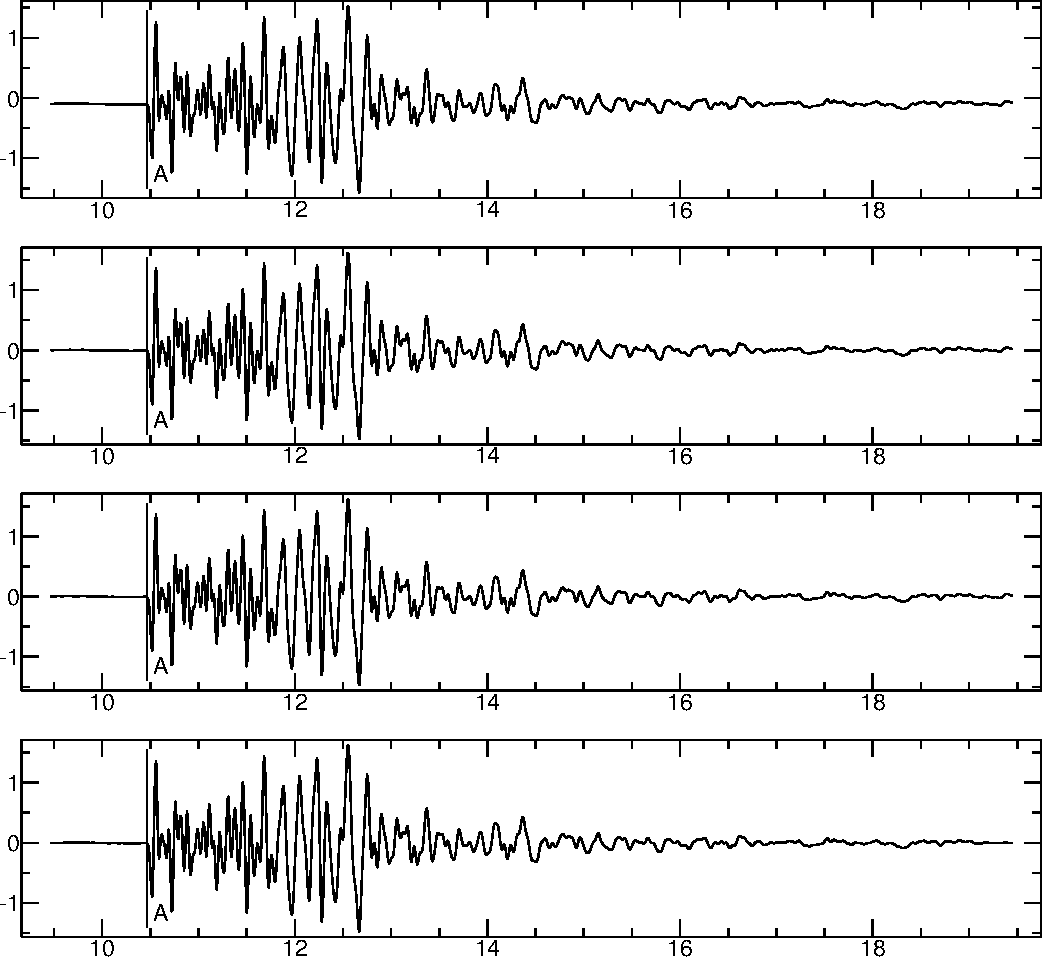
\includegraphics[width=0.9\textwidth]{rmean-rtrend-taper}
\caption{去均值、去线性趋势和波形尖灭}
\label{fig:rmean-rtrend-taper}
\end{figure}
